\documentclass{article} 

\usepackage[brazil]{babel}
\usepackage{enumitem}
\usepackage{amsmath}
\usepackage{booktabs}
\usepackage{bm}
\usepackage{float}
\usepackage[margin=2cm]{geometry}
\usepackage{circuitikz}
\usepackage{siunitx}
\usepackage{steinmetz}
\usepackage{amssymb}

\newcommand{\phasor}[2]{%
  #1 \, \phase{\, #2^\circ} \,
}

\newcommand{\ds}{\displaystyle}

% \newcommand{\phasor}[2]{%
%   #1 \, \text{\phase{\, \ang{#2}}} \,
% }

\newcommand{\nle}{%
  \notag \\[0pt]
}

\setlength{\parindent}{0pt}

\title{Modelagem Matemática da Microrrede CC} 
\author{} 
% \date{\today}
\date{}

\begin{document}

\maketitle

\section*{Esquemático da Microrrede CC}

\begin{figure}[h]
  \centering
  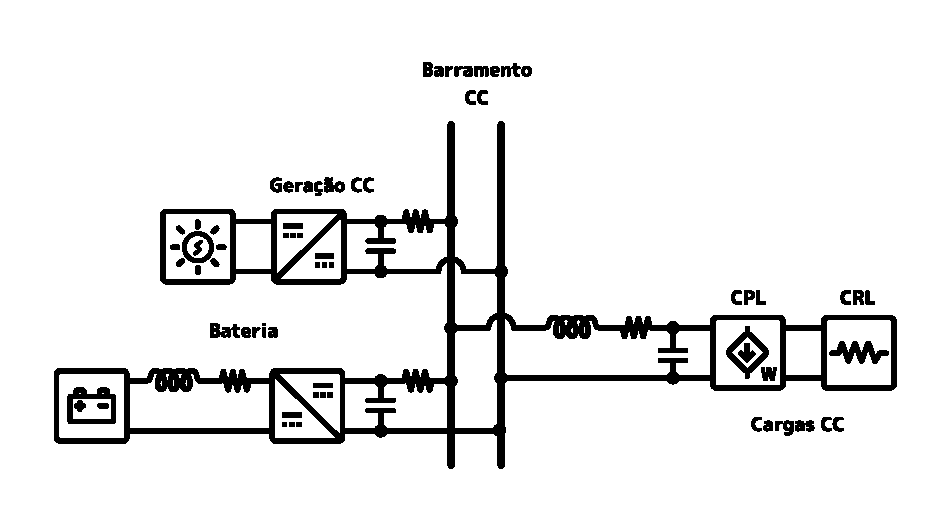
\includegraphics[width=14cm]{assets/dc_microgrid.eps}
  \caption{Esquemático da Microrrede CC}
  \label{fig:exemplo}
\end{figure}

\include{sections/nonlinear_model}


\end{document}
